%----------------------------------------------------------------------------
\chapter{Jegyzőkönyv}
%----------------------------------------------------------------------------

%----------------------------------------------------------------------------
\section{Első feladat}
%----------------------------------------------------------------------------
Első lépésként megnyitottuk a \textit{tank\_na\_m2017\_multi.slx} fájlt Simulink-kel. A kapcsoló segítségével átkapcsoltuk a rendszert a megadott PD szabályzóra és kipróbáltuk annak működését, mely a \figref{pd}~ábrán látható. A célunk hasonlóan működő rendszer(ek) megvalósítása a Fuzzy szabályzók segítségével.

\begin{figure}[!ht]
	\centering
	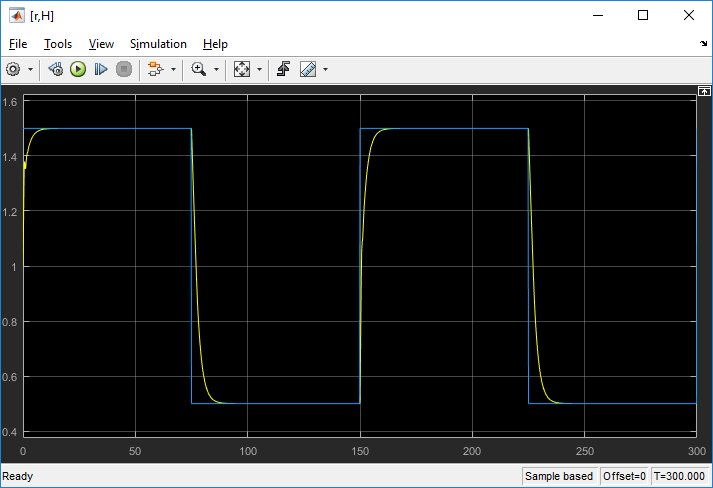
\includegraphics[width=150mm,keepaspectratio]{figures/m01/pd.png}
	\caption{Az alapjel és a PD szabályzóval kimenete, a vízszint} 
	\label{fig:pd}
\end{figure}

A Fuzzy Logic Toolbox segítségével létrehoztuk az először még üres szabályrendszert, Mamdani-féle implikációt választva. Bemenetként a vízszint hibáját és a vízszint változás sebességét adtuk meg, tagsági függvényeknek Gauss-eloszlást választottunk, melyet először a tartományon egyenletesen elosztva, azonos szórással próbáltunk elhelyezni. Így jártunk el a kimenetnél is, ám  ott már háromszög alakú tagsági függvényt használtunk. A bemeneteknél figyeltünk az átlapolódásra, mellyel elértük, hogy minden bemeneti értékre legyen válasza a rendszernek. A kimeneti tagsági függvényeket diszjunktnak választottuk, ezzel segítve a szabályzó döntését.

A szabályok megválasztásánál a MacVicar-Whelan metaszabályokat vettük alapul, először 3 kimeneti beavatkozás-változást előírva. A beállítások a \figref{FirstFuzzy}~ábrán láthatóak.

\begin{figure}[!h]
	\centering
	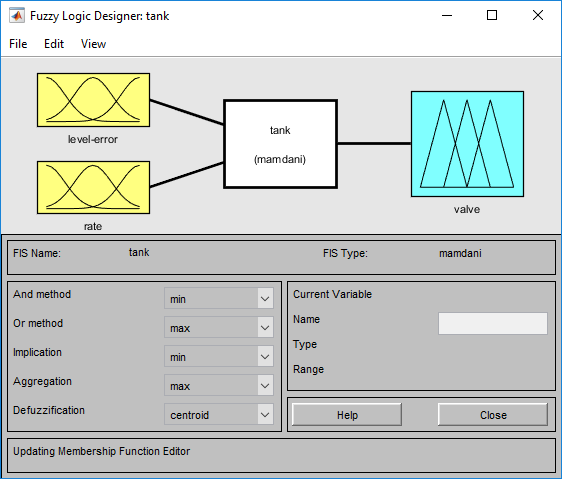
\includegraphics[width=71mm, keepaspectratio]{figures/m01/fuzzy1.png}\hspace{5mm}
	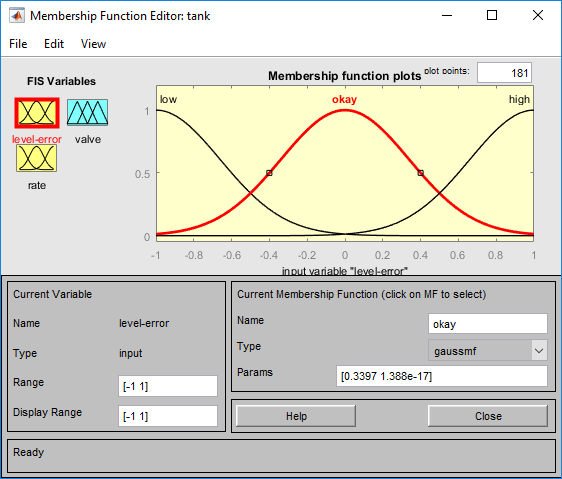
\includegraphics[width=71mm, keepaspectratio]{figures/m01/fuzzy2.png}\\\vspace{2.5mm}
	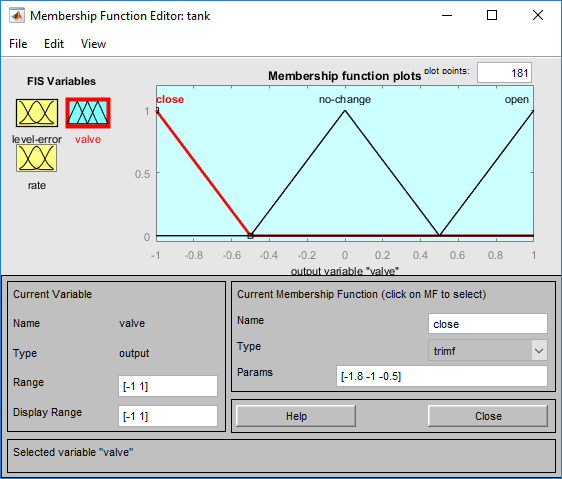
\includegraphics[width=71mm, keepaspectratio]{figures/m01/fuzzy3.png}\hspace{5mm}
	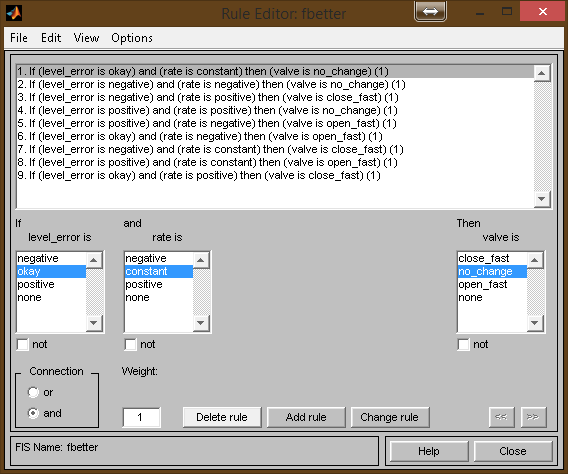
\includegraphics[width=71mm, keepaspectratio]{figures/m01/rules.png}
	%TODO ábraelnevezés
	\caption{A szabályzó megvalósítása a Fuzzy Logic Toolboxxal} 
	\label{fig:FirstFuzzy}
\end{figure}

Ezután Simulinkben visszaállítottuk a kapcsolót és leteszteltük a megvalósított Fuzzy szabályzót. Az alapjel, és a szabályzó kimenete, valamint a beavatkozó jel látható a \figref{FirstFuzzyResults}~ábrán láthatóak.

\begin{figure}[!h]
	\centering
	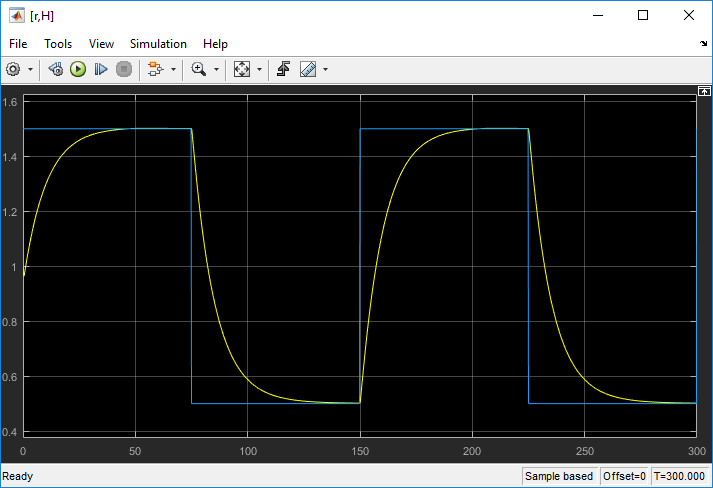
\includegraphics[width=71mm, keepaspectratio]{figures/m01/fuzzy4.png}\hspace{5mm}
	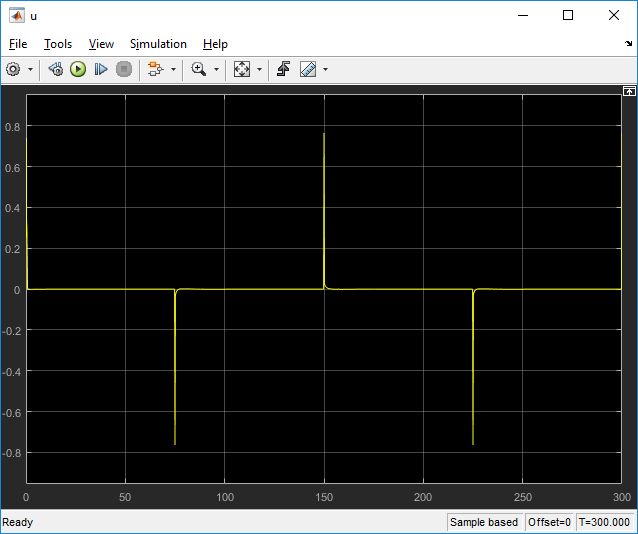
\includegraphics[width=71mm, keepaspectratio]{figures/m01/fuzzy5.png}
	%TODO ábraelnevezés
	\caption{A Fuzzy szabályzás eredménye} 
	\label{fig:FirstFuzzyResults}
\end{figure}
Az első verzió után több lehetőséget is kipróbáltunk, például több kimeneti tagsági függvényt, más eloszlásokat, azok elhelyezését, továbbá a T és S normákat változtatva se sikerült számottevő javulást elérni.

\newpage
%----------------------------------------------------------------------------
\section{Második feladat}
%----------------------------------------------------------------------------
A második feladatban a Fuzzy Toolboxban megtervezett szabályzó működését implementáltuk le. A program a beavatkozó jel meghatározása során a Fuzzy tagsági függvényeket \textit{0.01} raszterosztással értékeli ki, az éles numerikus értéket a \textit{Tömegközéppont-módszerrel} állítja elő. A programkód a Függelékben található, két megvalósított \textit{defuzzykálás} pedig a \figref{MatlabFuzzy}~ábrán.

\begin{figure}[!h]
	\centering
	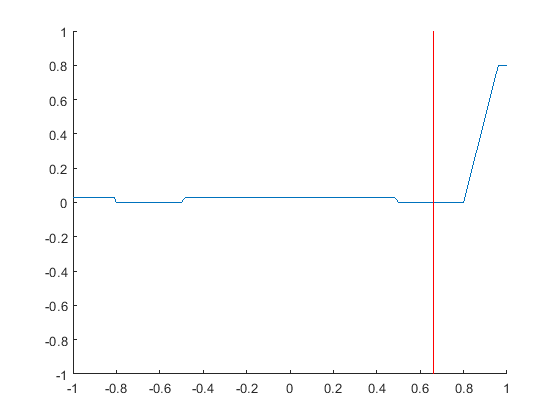
\includegraphics[width=71mm, keepaspectratio]{figures/m01/matlab2.png}\hspace{5mm}
	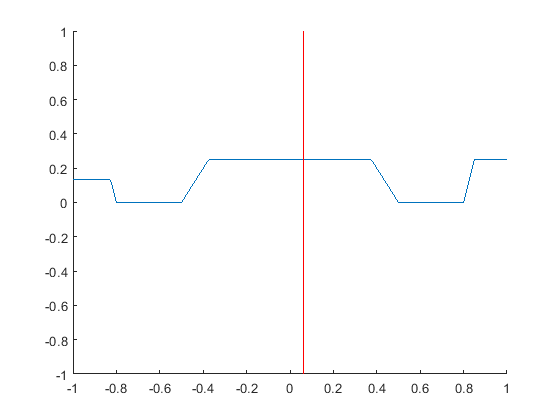
\includegraphics[width=71mm, keepaspectratio]{figures/m01/matlab3.png}
	%TODO ábraelnevezés
	\caption{Defuzzyfikálás} 
	\label{fig:MatlabFuzzy}
\end{figure}
A megfelelő kapcsolók beállításával leteszteltük az elkészített szabályzót, mely az eddigiekhez hasonlóan működött.

\begin{figure}
\centering
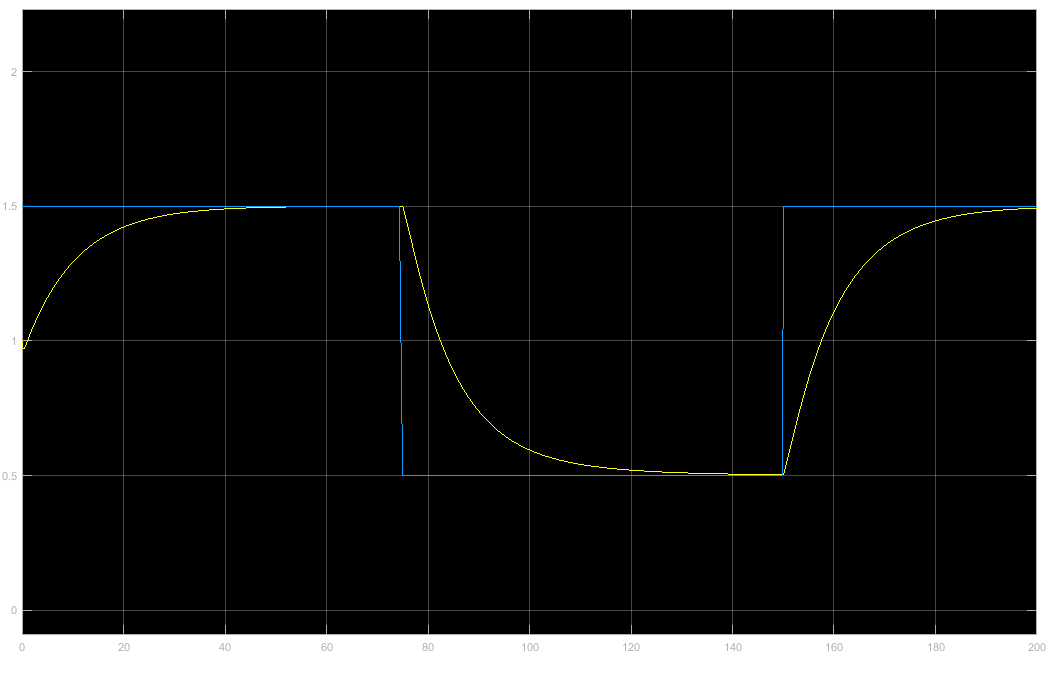
\includegraphics[width=131mm, keepaspectratio]{figures/m01/matlab1.png}
%TODO ábraelnevezés
\caption{A Fuzzy szabályzás eredménye} 
\label{fig:MatlabFuzzyResults}
\end{figure}
%----------------------------------------------------------------------------
\section{Konklúzió}
%----------------------------------------------------------------------------
Látható, hogy a PD szabályzó hatásfokát nem tudtuk elérni a fuzzy szabályzóval. Ennek az oka az, hogy a fuzzy szabálybázisunk csak kilenc szabályból állt. A bemenetei és kimenetei tartományokat több részre felosztva a fuzzy szabályzás pontosítható. A mérés során egyértelművé vált, hogy a fuzzy szabályzás a Matlab és azon belül is a Fuzzy Toolbox segítségével egyszerűen, átláthatóan elkészíthető.


